\documentclass[tikz]{standalone}
\usetikzlibrary{decorations.pathreplacing,calligraphy}
\begin{document}
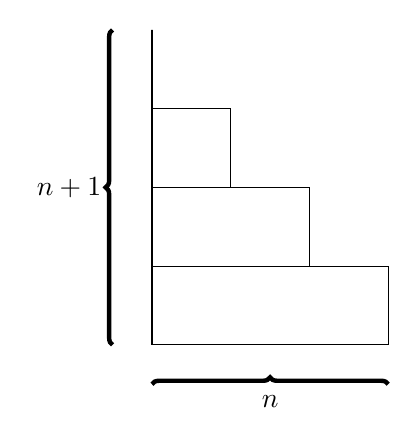
\begin{tikzpicture}[scale=1.0]
\draw[fill=white] (0, 0) rectangle (0, -1);
\draw[fill=white] (0, -1) rectangle (1, -2);
\draw[fill=white] (0, -2) rectangle (2, -3);
\draw[fill=white] (0, -3) rectangle (3, -4);

\draw[ultra thick, decorate, decoration={brace}] (-0.5, -4) -- node[left]{$n + 1$} (-0.5, 0);
\draw[ultra thick, decorate, decoration={brace}] (0, -4.5) -- node[below]{$n$} (3, -4.5);

\end{tikzpicture}
\end{document}